%!TEX root = ../main.tex

Dada la naturaleza geométrica del objeto a estudiar, la representación que resulta mas satisfactoria e intuitiva de ver en un principio de manera formal es la geométrica.

\begin{definition}
     Una \textbf{trenza geometrica} con $n\geq 1$ cuerdas es un conjunto $b\subset \R^2\times I$ formado por $n$ intervalos topológicos disyuntos llamados las \textit{cuerdas} de $b$, tales que la proyeccion $\R^2\times I\to I$, envia cada cuerda de manera homeomorfica a $I$, y ademas
     \begin{align*}
         b\cap(\R^2\times \{0\})=\{(i,0,0)|i=1,2,\ldots n\},\\
         b\cap(\R^2\times \{0\})=\{(i,0,1)|i=1,2,\ldots n\}.
     \end{align*}
\end{definition}
Observe que como cada cuerda va por medio de la proyección de manera homeomorfica a $I$, esto quiere decir que cada cuerda interseca a $\R^2\times\{t\}$ de manera única para cada $t\in I.$, es decir cada plano tiene exactamente $n$ puntos del conjunto $b.$ Note ademas que nuestra definición no menciona el punto final de cada una de las cuerdas ni el recorrido que hace. 
\begin{eg} El diagrama donde cada cuerda tiene como punto inicial y final el mismo y donde no hay ``giros''. 
    \begin{center}
    %!TEX root = ./main.tex

\tikzset{every picture/.style={line width=0.75pt}} %set default line width to 0.75pt        

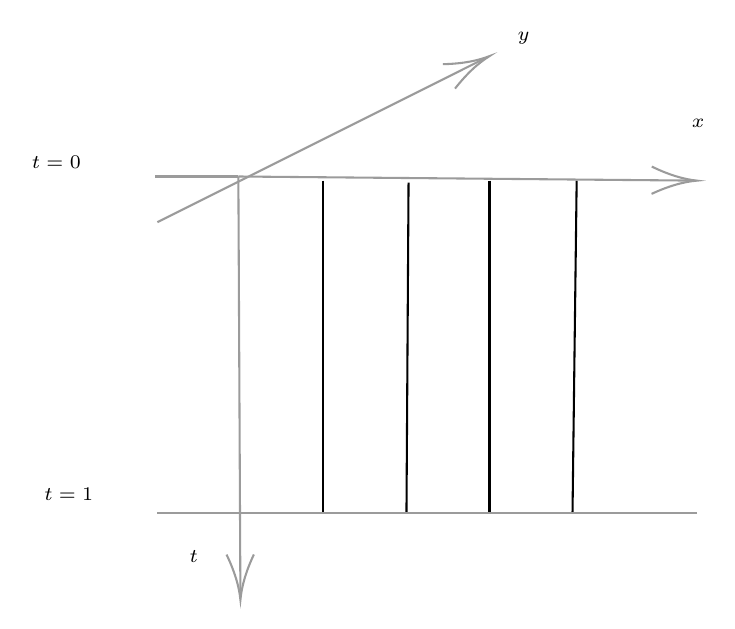
\begin{tikzpicture}[x=0.75pt,y=0.75pt,yscale=-2,xscale=2]
%uncomment if require: \path (0,300); %set diagram left start at 0, and has height of 300

%Straight Lines [id:da15571602795499961] 
\draw    (230,70) -- (230,150) ;
%Straight Lines [id:da6387164240227489] 
\draw    (250.5,70.5) -- (250,150) ;
%Straight Lines [id:da17127845146372145] 
\draw    (270,70) -- (270,150) ;
%Straight Lines [id:da1879833889944229] 
\draw    (291,70) -- (290,150) ;
%Straight Lines [id:da29818824665085064] 
\draw [color={rgb, 255:red, 155; green, 155; blue, 155 }  ,draw opacity=1 ]   (209.5,69) -- (209.99,169) ;
\draw [shift={(210,171)}, rotate = 269.72] [color={rgb, 255:red, 155; green, 155; blue, 155 }  ,draw opacity=1 ][line width=0.75]    (10.93,-3.29) .. controls (6.95,-1.4) and (3.31,-0.3) .. (0,0) .. controls (3.31,0.3) and (6.95,1.4) .. (10.93,3.29)   ;
%Straight Lines [id:da9999252093097876] 
\draw [color={rgb, 255:red, 155; green, 155; blue, 155 }  ,draw opacity=1 ]   (209.5,69) -- (318,69.98) ;
\draw [shift={(320,70)}, rotate = 180.52] [color={rgb, 255:red, 155; green, 155; blue, 155 }  ,draw opacity=1 ][line width=0.75]    (10.93,-3.29) .. controls (6.95,-1.4) and (3.31,-0.3) .. (0,0) .. controls (3.31,0.3) and (6.95,1.4) .. (10.93,3.29)   ;
%Straight Lines [id:da5087320786071492] 
\draw [color={rgb, 255:red, 155; green, 155; blue, 155 }  ,draw opacity=1 ]   (210,70) -- (268.21,40.89) ;
\draw [shift={(270,40)}, rotate = 153.43] [color={rgb, 255:red, 155; green, 155; blue, 155 }  ,draw opacity=1 ][line width=0.75]    (10.93,-3.29) .. controls (6.95,-1.4) and (3.31,-0.3) .. (0,0) .. controls (3.31,0.3) and (6.95,1.4) .. (10.93,3.29)   ;
%Straight Lines [id:da6250989615981395] 
\draw [color={rgb, 255:red, 155; green, 155; blue, 155 }  ,draw opacity=1 ]   (210,70) -- (190,80) ;
%Straight Lines [id:da8602700993161204] 
\draw [color={rgb, 255:red, 155; green, 155; blue, 155 }  ,draw opacity=1 ]   (209.5,69) -- (189.5,69) ;
%Straight Lines [id:da31711673101036175] 
\draw [color={rgb, 255:red, 155; green, 155; blue, 155 }  ,draw opacity=1 ]   (320,150) -- (190,150) ;

% Text Node
\draw (159,63.4) node [anchor=north west][inner sep=0.75pt]  [font=\scriptsize]  {$t=0$};
% Text Node
\draw (162,143.4) node [anchor=north west][inner sep=0.75pt]  [font=\scriptsize]  {$t=1$};
% Text Node
\draw (197,158.4) node [anchor=north west][inner sep=0.75pt]  [font=\scriptsize]  {$t$};
% Text Node
\draw (318,54.4) node [anchor=north west][inner sep=0.75pt]  [font=\scriptsize]  {$x$};
% Text Node
\draw (276,33.4) node [anchor=north west][inner sep=0.75pt]  [font=\scriptsize]  {$y$};


\end{tikzpicture}
    \end{center}
    Note que en este ejemplo sencillo si bien cada cuerda pareciera que se encuentra solo en el plano $(x,t)$, estas cuerdas se pueden deformar en la dirección del eje $y$, por lo que debemos ser cuidadosos con estas representaciones.
\end{eg}

\begin{eg}Observe que en este ejemplo los puntos iniciales y finales de cada cuerda son los mismos que el anterior, pero en este caso si hay cuerdas que ``giran'' al rededor de otras.
    \begin{center} 
        %!TEX root = ./main.tex

\tikzset{every picture/.style={line width=0.75pt}} %set default line width to 0.75pt        

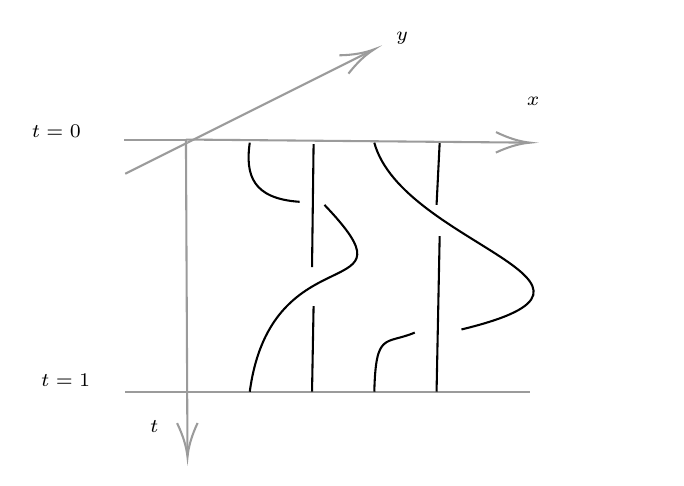
\begin{tikzpicture}[x=0.75pt,y=0.75pt,yscale=-1.5,xscale=1.5]
%uncomment if require: \path (0,300); %set diagram left start at 0, and has height of 300

%Straight Lines [id:da6387164240227489] 
\draw    (250.5,70.5) -- (250,110) ;
%Straight Lines [id:da1879833889944229] 
\draw    (291,70) -- (290,90) ;
%Straight Lines [id:da29818824665085064] 
\draw [color={rgb, 255:red, 155; green, 155; blue, 155 }  ,draw opacity=1 ]   (209.5,69) -- (209.99,169) ;
\draw [shift={(210,171)}, rotate = 269.72] [color={rgb, 255:red, 155; green, 155; blue, 155 }  ,draw opacity=1 ][line width=0.75]    (10.93,-3.29) .. controls (6.95,-1.4) and (3.31,-0.3) .. (0,0) .. controls (3.31,0.3) and (6.95,1.4) .. (10.93,3.29)   ;
%Straight Lines [id:da9999252093097876] 
\draw [color={rgb, 255:red, 155; green, 155; blue, 155 }  ,draw opacity=1 ]   (209.5,69) -- (318,69.98) ;
\draw [shift={(320,70)}, rotate = 180.52] [color={rgb, 255:red, 155; green, 155; blue, 155 }  ,draw opacity=1 ][line width=0.75]    (10.93,-3.29) .. controls (6.95,-1.4) and (3.31,-0.3) .. (0,0) .. controls (3.31,0.3) and (6.95,1.4) .. (10.93,3.29)   ;
%Straight Lines [id:da5087320786071492] 
\draw [color={rgb, 255:red, 155; green, 155; blue, 155 }  ,draw opacity=1 ]   (210,70) -- (268.21,40.89) ;
\draw [shift={(270,40)}, rotate = 153.43] [color={rgb, 255:red, 155; green, 155; blue, 155 }  ,draw opacity=1 ][line width=0.75]    (10.93,-3.29) .. controls (6.95,-1.4) and (3.31,-0.3) .. (0,0) .. controls (3.31,0.3) and (6.95,1.4) .. (10.93,3.29)   ;
%Straight Lines [id:da6250989615981395] 
\draw [color={rgb, 255:red, 155; green, 155; blue, 155 }  ,draw opacity=1 ]   (210,70) -- (190,80) ;
%Straight Lines [id:da8602700993161204] 
\draw [color={rgb, 255:red, 155; green, 155; blue, 155 }  ,draw opacity=1 ]   (209.5,69) -- (189.5,69) ;
%Straight Lines [id:da31711673101036175] 
\draw [color={rgb, 255:red, 155; green, 155; blue, 155 }  ,draw opacity=1 ]   (320,150) -- (190,150) ;
%Straight Lines [id:da7048848459711928] 
\draw    (250.5,122.5) -- (250,150) ;
%Curve Lines [id:da36065808527822485] 
\draw    (230,70) .. controls (228.5,80.5) and (231,88) .. (246,89) ;
%Curve Lines [id:da5874880850528349] 
\draw    (254,90) .. controls (285.5,123) and (237,98) .. (230,150) ;
%Curve Lines [id:da3625971369635478] 
\draw    (270,70) .. controls (279,103) and (360,115) .. (298,130) ;
%Straight Lines [id:da02942943718787716] 
\draw    (291,100) -- (290,150) ;
%Curve Lines [id:da5037121904515169] 
\draw    (270,150) .. controls (270.5,130.5) and (273.5,135) .. (283,131) ;

% Text Node
\draw (159,63.4) node [anchor=north west][inner sep=0.75pt]  [font=\scriptsize]  {$t=0$};
% Text Node
\draw (162,143.4) node [anchor=north west][inner sep=0.75pt]  [font=\scriptsize]  {$t=1$};
% Text Node
\draw (197,158.4) node [anchor=north west][inner sep=0.75pt]  [font=\scriptsize]  {$t$};
% Text Node
\draw (318,54.4) node [anchor=north west][inner sep=0.75pt]  [font=\scriptsize]  {$x$};
% Text Node
\draw (276,33.4) node [anchor=north west][inner sep=0.75pt]  [font=\scriptsize]  {$y$};


\end{tikzpicture}
    \end{center}
\end{eg}

A pesar de lo observado anteriormente los puntos finales e iniciales no tienen por que ser los mismos por lo que en general cada cuerda conectara a un  punto $(i,0,0)$ a un punto $(s(i),0,1)$, donde $i,s(i)\in\{1,2,\ldots n\}$.\\ 

Observe que la secuencia $(s(1),s(2),\ldots,s(n))$ es una permutacion del conjunto $\{1,2,\ldots, n\}$, por lo que para una trenza $b$ cualquiera, decimos que la secuencia $(s(1),s(2),\ldots,s(n))$ es la \textbf{permutacion subyacente} de $b$. En particular note que para los ejemplos anteriores tenemos la misma permutación subyacente $(1,2,3,4).$\\

Con esto en mente es natural preguntarse de que manera podemos ver si dos trenzas son ``equivalentes'' en algún sentido, para esto introducimos la noción de \textit{isotopia}.

\begin{definition}
    Dos trenzas $b$ y $b^\prime$ son isotopicas si existe una función continua $F:b\times I\to R^2\times I$, tal que para cada $s\in I$, la función $F_s:=F(-,s)$ es un embedimiento el cual su imagen es una trenza geométrica de $n$ cuerdas, $F_0=Id_b$ y $F_1(b)=b^\prime.$\\
    Tanto $F$ como la familia de trenzas geometricas $\{F_s(b)\}_{s\in I}$ se conocen como una isotopia de $b$ a $b^\prime$.
\end{definition}
Note que esta noción es muy parecida a una homotopia, asi naturalmente podemos verificar la siguiente propiedad.
\begin{prop}
    La isotopia entre trenzas geométricas define una relación de equivalencia.
\end{prop}
\begin{proof}
     \textcolor{blue}{luego}
\end{proof}
Dadas las similitudes con la noción de homotopia, podemos pensar en una forma de definir un ``producto'' trenzas geométricas con $n$ cuerdas.
\begin{definition}
    Dadas 2 trenzas geométricas con $n$ cuerdas $b_1,b_2$, definimos su producto como el conjunto de puntos $(x,y,t)\in \R^2\times I$ tales que si $t\in[0,1/2]$ entonces $(x,y,2t)\in b$, y en caso donde $t\in[1/2,1]$ tenemos que $(x,y,2t-1)\in b_2$.
\end{definition}
Note que el producto de dos trenzas geométricas de ese estilo claramente sera otra trenza, ya que lo único que estamos haciendo es unir el final de una con el inicio de la otra. La siguiente proposición nos permitirá definirla como un producto sobre las clases de trenzas geométricas con $n$ cuerdas
\begin{prop}
    Dadas $b_1,b_2,b_1^\prime,b_2^\prime$, donde $b_i$ es isotopica a $b_i^\prime$ para $i=1,2$, entonces $b_1b_2$ es isotopica a $b_1^\prime b^\prime_2$
\end{prop}
\begin{proof}
    \textcolor{blue}{luego}
\end{proof}
Dado esto podemos observar que esta operación es asociativa y ademas tiene un elemento neutro. Este elemento neutro sera denotado como $1_n$ y es presentador por la trenza geométrica dibujada de el ejemplo 2.2. en su expresión de conjunto seria
$$1_n=\{1,2,\ldots,n\}\times\{0\}\times I.$$
De esto concluimos que es un monoide, la prueba de que efectivamente resulta un grupo vendra mas adelante.
\subsection{Diagramas de Trenzas y movimientos de Reidemeister}
Como mencionamos en el Ejemplo 2.2, si bien uno debe ser cuidadoso con las representaciones, en términos prácticos esta proyección donde las cuerdas en el diagrama pareciera que están solo en el plano $y=0$ y donde lo tramos que pasan por ``debajo'' pareciera que se cortan son útiles, siempre y cuando de manera local solo hayan cortes transversales dos a dos. Esta idea nos lleva a querer definir estas representaciones.

\begin{definition}
    Un \textbf{diagrama de trenzas} de $n$ cuerdas es un conjunto $D\subset \R\times I$, vista como la union de $n$ intervalos topologicos llamados las cuerdas de $D$ donde se cumplen las siguientes condiciones.
    \begin{itemize}
        \item La proyeccion $\R\times I\to I$ envia cada cuerda homeomorficamente a $I.$
        \item Cada punto $\{1,2,\ldots\}\times\{0,1\}$ es el extremo de una unica cuerda.
        \item Todo punto de $\R\times I$ pertenece a lo maximo a 2 cuerdas. En cada punto de interseccion las cuerdas se cruzan de manera transversal y una de ellas se difumina para indicar que pasa por debajo, mientras la que se ve continua indica que pasa por arriba. 
        \end{itemize} 
\end{definition}
En particular si en los ejemplos 2.2 y 2.3 quitamos el eje $y$ serian diagramas de trenzas, pero incluimos la tercera condicion para evitar casos como el siguiente 
\begin{eg}
    Observe que en la figura es imposible distinguir que trenza pasa por debajo de la otra por lo que si bien podemos ver que la permutacion subyacente seria del tipo $(3,2,1)$ no sabemos como se comportan las trenzas por el dibujo.
    \begin{center}
    %!TEX root = ./main.tex


\tikzset{every picture/.style={line width=0.75pt}} %set default line width to 0.75pt        

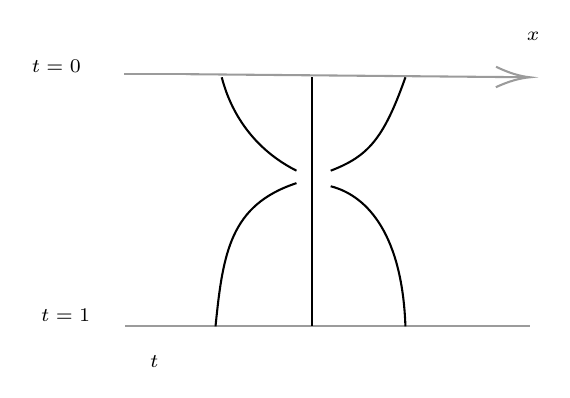
\begin{tikzpicture}[x=0.75pt,y=0.75pt,yscale=-1.5,xscale=1.5]
%uncomment if require: \path (0,300); %set diagram left start at 0, and has height of 300

%Straight Lines [id:da9999252093097876] 
\draw [color={rgb, 255:red, 155; green, 155; blue, 155 }  ,draw opacity=1 ]   (209.5,69) -- (318,69.98) ;
\draw [shift={(320,70)}, rotate = 180.52] [color={rgb, 255:red, 155; green, 155; blue, 155 }  ,draw opacity=1 ][line width=0.75]    (10.93,-3.29) .. controls (6.95,-1.4) and (3.31,-0.3) .. (0,0) .. controls (3.31,0.3) and (6.95,1.4) .. (10.93,3.29)   ;
%Straight Lines [id:da8602700993161204] 
\draw [color={rgb, 255:red, 155; green, 155; blue, 155 }  ,draw opacity=1 ]   (209.5,69) -- (189.5,69) ;
%Straight Lines [id:da31711673101036175] 
\draw [color={rgb, 255:red, 155; green, 155; blue, 155 }  ,draw opacity=1 ]   (320,150) -- (190,150) ;
%Straight Lines [id:da02070104769775316] 
\draw    (250,70) -- (250,150) ;
%Curve Lines [id:da05791226204824307] 
\draw    (221,70) .. controls (222.4,75.4) and (227.2,91) .. (245,100) ;
%Curve Lines [id:da40088925285683386] 
\draw    (280,70) .. controls (273,89.8) and (268,95.4) .. (256,100) ;
%Curve Lines [id:da876049615716019] 
\draw    (219,150) .. controls (221.4,126.2) and (223.8,111) .. (245,104) ;
%Curve Lines [id:da5837647469150872] 
\draw    (256,105) .. controls (268.4,108.2) and (279,121.4) .. (280,150) ;

% Text Node
\draw (159,63.4) node [anchor=north west][inner sep=0.75pt]  [font=\scriptsize]  {$t=0$};
% Text Node
\draw (162,143.4) node [anchor=north west][inner sep=0.75pt]  [font=\scriptsize]  {$t=1$};
% Text Node
\draw (197,158.4) node [anchor=north west][inner sep=0.75pt]  [font=\scriptsize]  {$t$};
% Text Node
\draw (318,54.4) node [anchor=north west][inner sep=0.75pt]  [font=\scriptsize]  {$x$};


\end{tikzpicture}
\end{center}
\end{eg}
La condicion en la que hemos realizado el particular enfasis, nos dice que via homeomorfismo en una vecindad de estos puntos de cruce, las trenzas se ven como el conjunto $\{(x,y):xy=0\}$ que en escencia son  los ejes coordenados de $\R^2.$\\

Otra implicacion de esta condicion es que el numero de cruces en $D  $ es finito, pues en caso contrario si fueran infinito (\textcolor{blue}{luego lo pienso}).\\

El proposito de introducir los diagramas de trenzas es que podemos ver como estos son representantes de la clase de isotopia de las trenzas geometricas de la manera mas natural posible. La idea detrás de esto es ver a el diagrama de trenzas de la manera natural dentro de $\R^2\times I$, como $\R\times\{0\}\times I$, asi en cada vecindad de intersección cambiamos la coordenada de la trenza que pasa por debajo mientras las otras dos las dejamos quietas, es decir nuestra cuerda ahora se encontrara ubicada en $\R\times(0,\infty)\times I.$ Este acto que es continuo y transforma el diagrama $D$ en una trenza geométrica, la cual tiene su clase de isotopia bien definida presentada por $D$, esto suele denotarse por $\beta(D).$\\

Con esto en mente es relativamente sencillo imaginarse la forma en la que uno puede transformar un elemento de la clase de isotopia en un diagrama, dada $\beta$ una trenza geométrica, en la clase de isotopia podemos encontrar una trenza geométrica $b$ donde solo se den los cruces de manera transversal, luego si recordamos cuales son las cuerdas que tienen segunda coordenada mas grande en el corte al momento de hacer la proyección $\R^2\times I\to R\times{0}\times I$ estas serán en las que tomaremos sub-arcos de $b$ para que se vea ``cortada'', de esta manera podemos obtener el diagrama $D$ que es claramente igual a $\beta(D).$ Con esta idea de que podemos pasar libre mente de la trenza geométrica a un diagrama de trenzas pues debemos de definir que es la isotopia en estos diagramas.
\begin{definition}
     Dos diagramas de trenzas $D$ y $D^\prime$ se dicen isotopicos  si existe una funcion continua $F:D\times I\to R\times I$ tal que para cada $s\in I$, $D_s=F(D\times\{s\})\subset \R\times I$ es un diagrama de trenzas con la misma cantidad cuerdas, ademas $D_0=D$ y $D_1=D^\prime.$ 
 \end{definition} 
 Se sobreentiende de la definición de que la función $F$ en cada $s$ envía los cruces y la información de quien va por debajo y arriba a $D_s$.
 \begin{eg}
     Observe que podemos ver todo lo que se menciono antes, la información se preserva tanto de los cortes como de que cuerda va por debajo.
     \begin{center}
    
%!TEX root = ./main.tex

\tikzset{every picture/.style={line width=0.75pt}} %set default line width to 0.75pt        

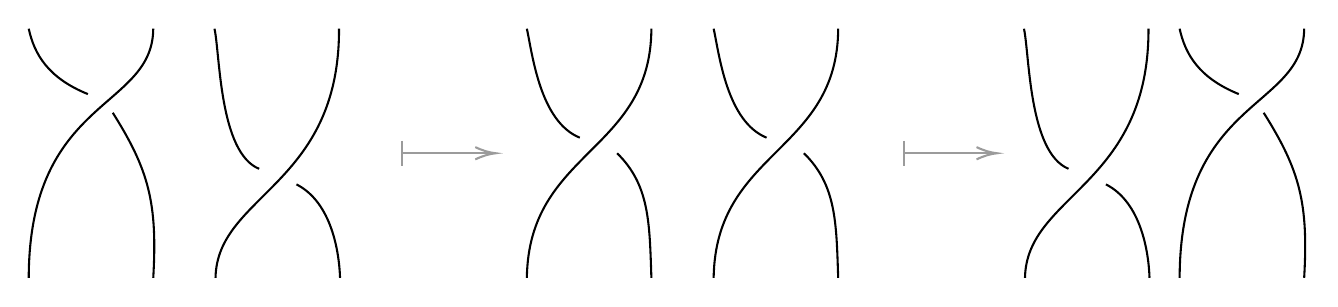
\begin{tikzpicture}[x=0.75pt,y=0.75pt,yscale=-1.5,xscale=1.5]
%uncomment if require: \path (0,300); %set diagram left start at 0, and has height of 300

%Curve Lines [id:da467535346440173] 
\draw    (100,100) .. controls (101.8,108.2) and (106.2,115.8) .. (119,121) ;
%Curve Lines [id:da18360277031656336] 
\draw    (140,100) .. controls (139.8,126.2) and (100.2,121.8) .. (100,180) ;
%Curve Lines [id:da8935762898756716] 
\draw    (127,127) .. controls (138.6,145.4) and (141.4,156) .. (140,180) ;
%Curve Lines [id:da11204595747175461] 
\draw    (159.67,100) .. controls (161.47,108.2) and (161.2,139.8) .. (174,145) ;
%Curve Lines [id:da9612794099188988] 
\draw    (199.67,100) .. controls (199.8,150.6) and (160.53,153.2) .. (160,180) ;
%Curve Lines [id:da9839227280377414] 
\draw    (186,150) .. controls (197.4,155.8) and (199.73,172) .. (200,180) ;
%Straight Lines [id:da021068853778946184] 
\draw [color={rgb, 255:red, 155; green, 155; blue, 155 }  ,draw opacity=1 ]   (220,140) -- (248,140) ;
\draw [shift={(250,140)}, rotate = 180] [color={rgb, 255:red, 155; green, 155; blue, 155 }  ,draw opacity=1 ][line width=0.75]    (6.56,-1.97) .. controls (4.17,-0.84) and (1.99,-0.18) .. (0,0) .. controls (1.99,0.18) and (4.17,0.84) .. (6.56,1.97)   ;
%Straight Lines [id:da95151298393968] 
\draw [color={rgb, 255:red, 155; green, 155; blue, 155 }  ,draw opacity=1 ]   (220,136) -- (220,144) ;
%Curve Lines [id:da5609149547400984] 
\draw    (260,100) .. controls (261.8,108.2) and (264.2,129.8) .. (277,135) ;
%Curve Lines [id:da2754758327066825] 
\draw    (300,100) .. controls (299.8,139.8) and (260.6,139) .. (260,180) ;
%Curve Lines [id:da8793140836193352] 
\draw    (289,140) .. controls (299.4,150.2) and (299.4,162.2) .. (300,180) ;
%Curve Lines [id:da24663066435532877] 
\draw    (320,100) .. controls (321.8,108.2) and (324.2,129.8) .. (337,135) ;
%Curve Lines [id:da0768559780876632] 
\draw    (360,100) .. controls (359.8,139.8) and (320.6,139) .. (320,180) ;
%Curve Lines [id:da2528200653455043] 
\draw    (349,140) .. controls (359.4,150.2) and (359.4,162.2) .. (360,180) ;
%Straight Lines [id:da4894361551183606] 
\draw [color={rgb, 255:red, 155; green, 155; blue, 155 }  ,draw opacity=1 ]   (381,140) -- (409,140) ;
\draw [shift={(411,140)}, rotate = 180] [color={rgb, 255:red, 155; green, 155; blue, 155 }  ,draw opacity=1 ][line width=0.75]    (6.56,-1.97) .. controls (4.17,-0.84) and (1.99,-0.18) .. (0,0) .. controls (1.99,0.18) and (4.17,0.84) .. (6.56,1.97)   ;
%Straight Lines [id:da5885887633516773] 
\draw [color={rgb, 255:red, 155; green, 155; blue, 155 }  ,draw opacity=1 ]   (381,136) -- (381,144) ;
%Curve Lines [id:da58316887037238] 
\draw    (469.67,100) .. controls (471.47,108.2) and (475.87,115.8) .. (488.67,121) ;
%Curve Lines [id:da5892164363370944] 
\draw    (509.67,100) .. controls (509.47,126.2) and (469.87,121.8) .. (469.67,180) ;
%Curve Lines [id:da37395946502444233] 
\draw    (496.67,127) .. controls (508.27,145.4) and (511.07,156) .. (509.67,180) ;
%Curve Lines [id:da857579069977218] 
\draw    (419.67,100) .. controls (421.47,108.2) and (421.2,139.8) .. (434,145) ;
%Curve Lines [id:da8117026709461808] 
\draw    (459.67,100) .. controls (459.8,150.6) and (420.53,153.2) .. (420,180) ;
%Curve Lines [id:da2598178790696365] 
\draw    (446,150) .. controls (457.4,155.8) and (459.73,172) .. (460,180) ;




\end{tikzpicture}
\end{center}
 \end{eg}
 Análogamente el producto de diagramas $D_1$ y $D_2$ lo podemos ver como pegar un diagrama encima de otro para posteriormente aplastarlo hasta que este contenido en $\R\times I,$ ese producto sera llamado $D_1D_2$ y este diagrama representara el producto de las trenzas $\beta_1$ y $\beta_2$ correspondientes
 \begin{eg} El producto de dos diagramas para obtener $D_1D_2$ y $D_2D_1$
     \begin{center}
         %!TEX root = ./main.tex



\tikzset{every picture/.style={line width=0.75pt}} %set default line width to 0.75pt        

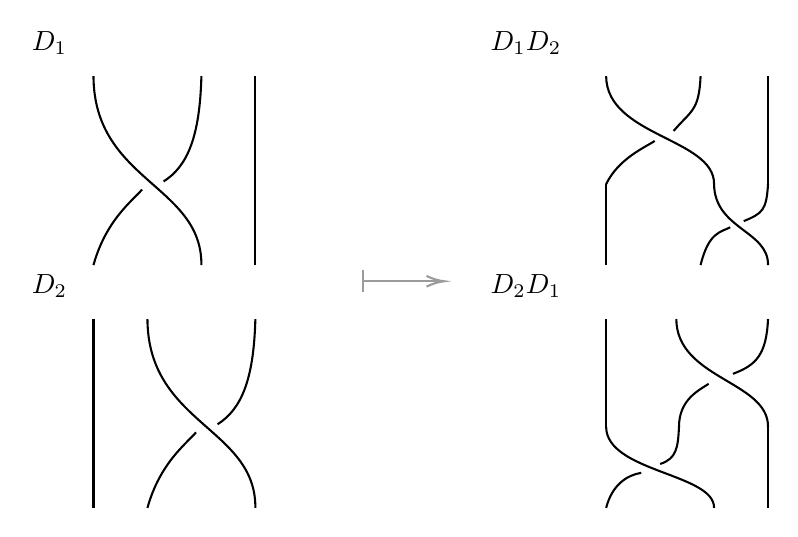
\begin{tikzpicture}[x=0.75pt,y=0.75pt,yscale=-1.3,xscale=1.3]
%uncomment if require: \path (0,300); %set diagram left start at 0, and has height of 300

%Straight Lines [id:da021068853778946184] 
\draw [color={rgb, 255:red, 155; green, 155; blue, 155 }  ,draw opacity=1 ]   (170,146) -- (198,146) ;
\draw [shift={(200,146)}, rotate = 180] [color={rgb, 255:red, 155; green, 155; blue, 155 }  ,draw opacity=1 ][line width=0.75]    (6.56,-1.97) .. controls (4.17,-0.84) and (1.99,-0.18) .. (0,0) .. controls (1.99,0.18) and (4.17,0.84) .. (6.56,1.97)   ;
%Straight Lines [id:da95151298393968] 
\draw [color={rgb, 255:red, 155; green, 155; blue, 155 }  ,draw opacity=1 ]   (170,142) -- (170,150) ;
%Curve Lines [id:da267445420900821] 
\draw    (70,70) .. controls (70.2,109) and (110.2,110.2) .. (110,140) ;
%Curve Lines [id:da9560126881859321] 
\draw    (110,70) .. controls (109.4,92.6) and (104.8,103.4) .. (96,109) ;
%Curve Lines [id:da69932409686339] 
\draw    (70,140) .. controls (74.6,123.4) and (84.4,116.2) .. (88,112) ;
%Straight Lines [id:da3984579751574062] 
\draw    (130,70) -- (130,140) ;
%Curve Lines [id:da9275419139907757] 
\draw    (90,160) .. controls (90.2,199) and (130.2,200.2) .. (130,230) ;
%Curve Lines [id:da7634162233242681] 
\draw    (130,160) .. controls (129.4,182.6) and (124.8,193.4) .. (116,199) ;
%Curve Lines [id:da3594253594620098] 
\draw    (90,230) .. controls (94.6,213.4) and (104.4,206.2) .. (108,202) ;
%Straight Lines [id:da8993733494160759] 
\draw    (70,160) -- (70,230) ;
%Curve Lines [id:da3504419970988496] 
\draw    (260,70) .. controls (260.2,92.29) and (300.2,92.97) .. (300,110) ;
%Curve Lines [id:da858985711627] 
\draw    (295,70) .. controls (294.4,82.91) and (291.6,82.6) .. (285,90.29) ;
%Curve Lines [id:da617506159593737] 
\draw    (260,110) .. controls (264.6,100.51) and (274.4,96.4) .. (278,94) ;
%Straight Lines [id:da6443868731225134] 
\draw    (320,70) -- (320,110) ;
%Curve Lines [id:da9288543035495236] 
\draw    (300,110) .. controls (300.2,126.71) and (320.2,127.23) .. (320,140) ;
%Curve Lines [id:da16812105145415968] 
\draw    (320,110) .. controls (319.4,119.69) and (318,120.8) .. (311,123.71) ;
%Curve Lines [id:da5422492381478998] 
\draw    (295,140) .. controls (298,127.8) and (302.4,127.8) .. (306,126) ;
%Straight Lines [id:da0187639766750477] 
\draw    (260,110) -- (260,140) ;
%Curve Lines [id:da7389794431084341] 
\draw    (286,160) .. controls (286.2,182.29) and (320.2,182.97) .. (320,200) ;
%Curve Lines [id:da6936020178428224] 
\draw    (320,160) .. controls (319.4,172.91) and (315.8,177.09) .. (307,180.29) ;
%Curve Lines [id:da18137766551243817] 
\draw    (287,200) .. controls (287,189.8) and (294.4,186.4) .. (298,184) ;
%Straight Lines [id:da9358369635636983] 
\draw    (260,160) -- (260,200) ;
%Curve Lines [id:da9019075794007094] 
\draw    (260,200) .. controls (260.2,216.71) and (300.2,217.23) .. (300,230) ;
%Curve Lines [id:da39127651703057165] 
\draw    (287,200) .. controls (286.6,207.4) and (286.2,211.8) .. (280,213.71) ;
%Curve Lines [id:da8806113468711441] 
\draw    (260,230) .. controls (262.2,221.4) and (267.8,217.8) .. (273,217) ;
%Straight Lines [id:da20734068021017715] 
\draw    (320,200) -- (320,230) ;

% Text Node
\draw (46,52.4) node [anchor=north west][inner sep=0.75pt]    {$D_{1}$};
% Text Node
\draw (46,142.4) node [anchor=north west][inner sep=0.75pt]    {$D_{2}$};
% Text Node
\draw (216,52.4) node [anchor=north west][inner sep=0.75pt]    {$D_{1} D_{2}$};
% Text Node
\draw (216,142.4) node [anchor=north west][inner sep=0.75pt]    {$D_{2} D_{1}$};


\end{tikzpicture}

     \end{center}
 \end{eg}
 Note que esto ya nos muestra la no conmutatividad ya que la permutacion subyacente de el representante $D_1D_2$ es $(3,1,2)$, mientras que la de $D_2D_1$ es $(2,3,1).$\\

 Por ultimo, teniendo en cuenta que todos los diagramas los podemos pensar como cuerdas en la realidad es natural pensar en que movimientos preservan la clase de isotopia entre diagramas, para esto tomamos prestados de la teoria de nudos los \textit{movimientos de Reidemeister} $\Omega_2$ y $\Omega_3$
 \begin{definition}
 Definimos $\Omega_2$ un movimiento donde tomamos dos cuerdas del diagrama y creamos dos cruces nuevos transversales, pasando una de las cuerdas del diagrama por debajo de la otra, mientras que a $\Omega_3$ es un movimiento que involucra a tres cuerdas y preserva el numero de cruces transversales pero invierte el diagrama de manera reflexiva.  
 \end{definition}

 Estos movimientos solo afectan el diagrama en un disco dentro de $\R\times I$ y podemos verlos a continuación
 \begin{center}
     

\tikzset{every picture/.style={line width=0.75pt}} %set default line width to 0.75pt        

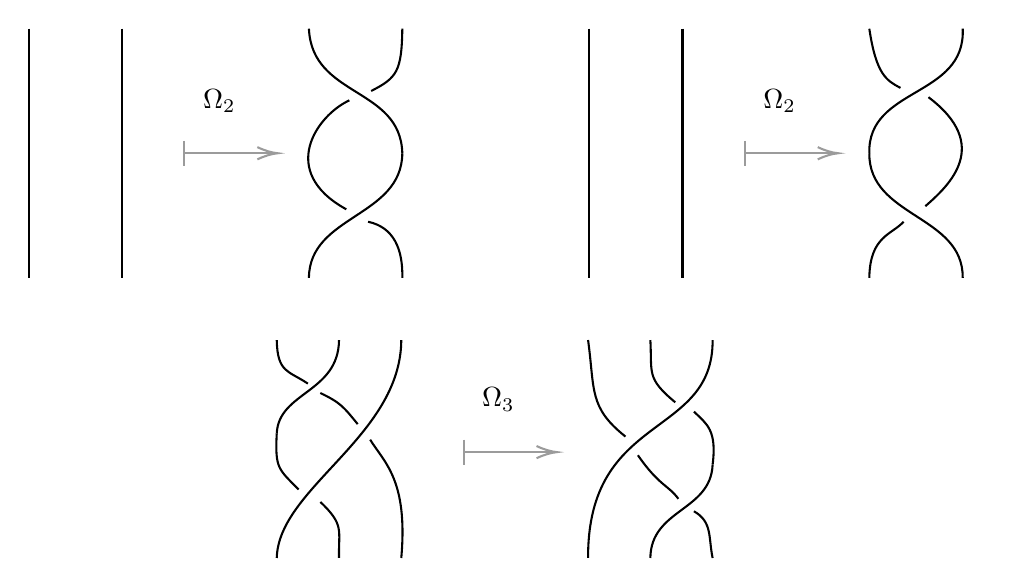
\begin{tikzpicture}[x=0.75pt,y=0.75pt,yscale=-1.5,xscale=1.5]
%uncomment if require: \path (0,300); %set diagram left start at 0, and has height of 300

%Straight Lines [id:da021068853778946184] 
\draw [color={rgb, 255:red, 155; green, 155; blue, 155 }  ,draw opacity=1 ]   (80,120) -- (108,120) ;
\draw [shift={(110,120)}, rotate = 180] [color={rgb, 255:red, 155; green, 155; blue, 155 }  ,draw opacity=1 ][line width=0.75]    (6.56,-1.97) .. controls (4.17,-0.84) and (1.99,-0.18) .. (0,0) .. controls (1.99,0.18) and (4.17,0.84) .. (6.56,1.97)   ;
%Straight Lines [id:da95151298393968] 
\draw [color={rgb, 255:red, 155; green, 155; blue, 155 }  ,draw opacity=1 ]   (80,116) -- (80,124) ;
%Straight Lines [id:da3105397663180821] 
\draw    (30,80) -- (30,160) ;
%Straight Lines [id:da41257341713042317] 
\draw    (60,80) -- (60,160) ;
%Curve Lines [id:da11900760040973013] 
\draw    (150,120) .. controls (149.8,140.6) and (120.2,139.8) .. (120,160) ;
%Curve Lines [id:da21344602026956538] 
\draw    (120,80) .. controls (121,102.2) and (149.4,98.6) .. (150,120) ;
%Curve Lines [id:da9689941604419631] 
\draw    (150,80) .. controls (149.8,93.8) and (148.2,95.8) .. (140,100) ;
%Curve Lines [id:da6960165665741206] 
\draw    (133,103) .. controls (122.6,107.8) and (109.8,125.8) .. (132,138) ;
%Curve Lines [id:da16812588273365814] 
\draw    (139,142) .. controls (147.4,143.8) and (150.2,151) .. (150,160) ;
%Straight Lines [id:da8993877656078348] 
\draw [color={rgb, 255:red, 155; green, 155; blue, 155 }  ,draw opacity=1 ]   (259.99,120) -- (287.99,120) ;
\draw [shift={(289.99,120)}, rotate = 180] [color={rgb, 255:red, 155; green, 155; blue, 155 }  ,draw opacity=1 ][line width=0.75]    (6.56,-1.97) .. controls (4.17,-0.84) and (1.99,-0.18) .. (0,0) .. controls (1.99,0.18) and (4.17,0.84) .. (6.56,1.97)   ;
%Straight Lines [id:da3147593233270113] 
\draw [color={rgb, 255:red, 155; green, 155; blue, 155 }  ,draw opacity=1 ]   (259.99,116) -- (259.99,124) ;
%Straight Lines [id:da36120199173040735] 
\draw    (209.99,80) -- (209.99,160) ;
%Straight Lines [id:da767115805534779] 
\draw    (239.99,80) -- (239.99,160) ;
%Curve Lines [id:da44641148036727185] 
\draw    (300,120) .. controls (299.8,140.6) and (330.2,139.8) .. (330,160) ;
%Curve Lines [id:da6320743672082285] 
\draw    (330,80) .. controls (331,102.2) and (299.4,98.6) .. (300,120) ;
%Curve Lines [id:da6313849027023718] 
\draw    (311,142) .. controls (307.2,146.2) and (300.2,146.6) .. (300,160) ;
%Curve Lines [id:da0589500737742894] 
\draw    (319,102) .. controls (339.4,117.4) and (325.8,130.2) .. (318,137) ;
%Curve Lines [id:da7255177605237971] 
\draw    (310,99) .. controls (305.4,96.6) and (302.2,94.6) .. (300,80) ;
%Curve Lines [id:da23638349304952366] 
\draw    (149.67,180) .. controls (149.47,211) and (110.27,227.4) .. (109.67,250) ;
%Curve Lines [id:da8983550529947678] 
\draw    (129.67,180) .. controls (129.47,197) and (110.27,196.6) .. (109.67,210) ;
%Curve Lines [id:da5344052460604444] 
\draw    (109.67,210) .. controls (109.07,221.4) and (110.27,221.4) .. (116.67,228) ;
%Curve Lines [id:da9058141972471662] 
\draw    (129.67,250) .. controls (129.47,241) and (131.47,239.4) .. (123.67,232) ;
%Curve Lines [id:da1999229819183379] 
\draw    (109.67,180) .. controls (109.87,190.6) and (113.47,189.8) .. (119.67,194) ;
%Curve Lines [id:da5382611206991912] 
\draw    (123.67,197) .. controls (130.27,200.2) and (131.07,201.4) .. (135.67,207) ;
%Curve Lines [id:da9383909926867282] 
\draw    (139.67,212) .. controls (144.27,219.4) and (151.87,225) .. (149.67,250) ;
%Straight Lines [id:da9655390534837395] 
\draw [color={rgb, 255:red, 155; green, 155; blue, 155 }  ,draw opacity=1 ]   (169.67,216) -- (197.67,216) ;
\draw [shift={(199.67,216)}, rotate = 180] [color={rgb, 255:red, 155; green, 155; blue, 155 }  ,draw opacity=1 ][line width=0.75]    (6.56,-1.97) .. controls (4.17,-0.84) and (1.99,-0.18) .. (0,0) .. controls (1.99,0.18) and (4.17,0.84) .. (6.56,1.97)   ;
%Straight Lines [id:da030621442854791958] 
\draw [color={rgb, 255:red, 155; green, 155; blue, 155 }  ,draw opacity=1 ]   (169.67,212) -- (169.67,220) ;
%Curve Lines [id:da5794729440142999] 
\draw    (249.67,180) .. controls (249.87,211.8) and (209.47,203) .. (209.67,250) ;
%Curve Lines [id:da10826159713872396] 
\draw    (229.67,180) .. controls (230.27,190.6) and (228.27,192.2) .. (237.67,200) ;
%Curve Lines [id:da991680044584273] 
\draw    (229.67,250) .. controls (229.87,234.2) and (249.07,235) .. (249.67,220) ;
%Curve Lines [id:da7350174882368962] 
\draw    (243.67,203) .. controls (247.87,207) and (251.07,209) .. (249.67,220) ;
%Curve Lines [id:da9744338524826922] 
\draw    (209.67,180) .. controls (211.87,196.2) and (209.87,201.6) .. (221.67,211) ;
%Curve Lines [id:da1740724973590062] 
\draw    (243.67,235) .. controls (249.67,238.4) and (248.27,243.4) .. (249.67,250) ;
%Curve Lines [id:da3320368868474375] 
\draw    (225.67,217) .. controls (232.47,226.8) and (235.47,226.6) .. (238.67,231) ;

% Text Node
\draw (85,98.4) node [anchor=north west][inner sep=0.75pt]    {$\Omega _{2}$};
% Text Node
\draw (264.99,98.4) node [anchor=north west][inner sep=0.75pt]    {$\Omega _{2}$};
% Text Node
\draw (174.67,194.4) node [anchor=north west][inner sep=0.75pt]    {$\Omega _{3}$};


\end{tikzpicture}
 \end{center}
 Decimos que el movimiento inverso es invertir las flechas en la figura, note que esto nos permite jugar con las cuerdas sin cambiar la estructura del diagrama, por lo que podemos definir una nocion de equivalencia
 \begin{definition}
     Dados dos diagramas $D$ y $D^\prime$ decimos que son $R$-equivalentes si $D$ se puede transformas por medio de una secuencia finita de isotopias y movimientos de Reidemeister a $D^\prime$
 \end{definition}
 A simple instancia no parece tan claro que esta nocion de equivalencia pueda ser trasladada hacia todas las trenzas geométricas, pero resulta que si podemos hacerlo
 \begin{theorem}
     Dos diagramas de trenzas representan trenzas geométricas isotopicas si y solo si estos diagramas son $R$-equivalentes.
 \end{theorem}
 La prueba de este hecho se reduce a cuatro pasos, pero la terminología y longitud de la prueba se salen de los propósitos del proyecto, para la prueba de este hecho vea \cite{KasselTuraev2008}.





